
\part{eu acuso!}



\chapter[Eu acuso!,\\ por Émile Zola]{eu acuso!\subtitulo{por Émile Zola}}
\hedramarkboth{Eu acuso!}{Zola}

\section{carta a m.~félix faure,\break presidente da república}

Excelentíssimo senhor Presidente da República, 
permita-me, em gratidão à generosa acolhida que o senhor me deu em
uma ocasião passada, apelar para a sua justa glória e dizer que sua
estrela, tão honrada até aqui, está ameaçada pela maior das vergonhas,
a mais indelével das manchas.

O senhor livrou-se, são e salvo, das maiores calúnias, tendo
conquistado os corações; saiu apoteótica e radiosamente desta festa
patriótica que foi para a França a aliança com a Rússia, e prepara-se
para presidir ao triunfo solene da nossa Exposição Universal, que
coroará nosso grande século cheio de trabalho, verdade e liberdade. Mas
é enorme a mancha sob o seu nome --- eu iria dizer sob seu governo --- que
é esse abominável caso Dreyfus! Uma corte marcial acaba, por ter
recebido ordens nesse sentido, de ousar absolver o tal Esterhazy,
supremo golpe em qualquer verdade, em qualquer justiça. E está feito: a
vergonha está estampada no rosto da França, e a história registrará que
foi sob a sua presidência que tamanho crime social foi cometido.

 E como foram ousados, serei da minha parte ousado também. Vou falar a
verdade, pois prometi resguardá-la, já que a justiça, conspurcada
diversas vezes, não faz isso, plena e inteiramente. Tenho o dever de
falar, eu não quero ser cúmplice. Minhas noites seriam assombradas pelo
espectro de um inocente que sofre no além-mar, mergulhado na mais
dolorosa tortura, por um crime que ele não cometeu.

E será à Sua Excelência, senhor Presidente, que dirigirei meus
clamores, a verdade, com toda a força da minha revolta de homem
honesto. Conheço a sua honra e, por isso, sei que ignora a verdade. A 
quem mais eu poderia denunciar a turba malfeitora dos verdadeiros
culpados, que não à Sua Excelência, o primeiro magistrado do país?

 A verdade, para começar, sobre o processo e a condenação de Dreyfus.

 Um homem nefasto, responsável por tudo, autor de tudo, é o comandante
du Paty de Clam, naquele momento um simples oficial. Ele é a
personificação do caso Dreyfus; nada será esclarecido até que uma
investigação imparcial tenha estabelecido claramente seus atos e sua
responsabilidade. Ele representa uma figura nebulosa, a mais complicada,
obcecado pelas intrigas romanescas, comprazendo-se, à maneira dos folhetins
baratos, com papéis que desaparecem, cartas anônimas, encontros em
lugares desertos, mulheres misteriosas que carregam, à noite, provas
irrefutáveis. Ele imagina ter ditado o documento a Dreyfus; é ele que
sonha estudá-lo em um cômodo inteiramente revestido de espelhos, é
ele que o comandante Forzinetti nos representa, empunhando uma lanterna
velada, desejando se aproximar do acusado adormecido, para projetar
sobre seus olhos um jato de luz e surpreendê-lo então em seu crime,
na confusão do sonho. Não tenho mais nada a dizer: se procurar, alguma
coisa aparece. Declaro simplesmente que o comandante du Paty de Clam,
encarregado de instruir o caso Dreyfus, como representante da justiça,
e, segundo a cronologia e a importância dos fatos, é o primeiro culpado
do erro judicial que foi cometido.

\begin{figure}
\centering
\clearpage
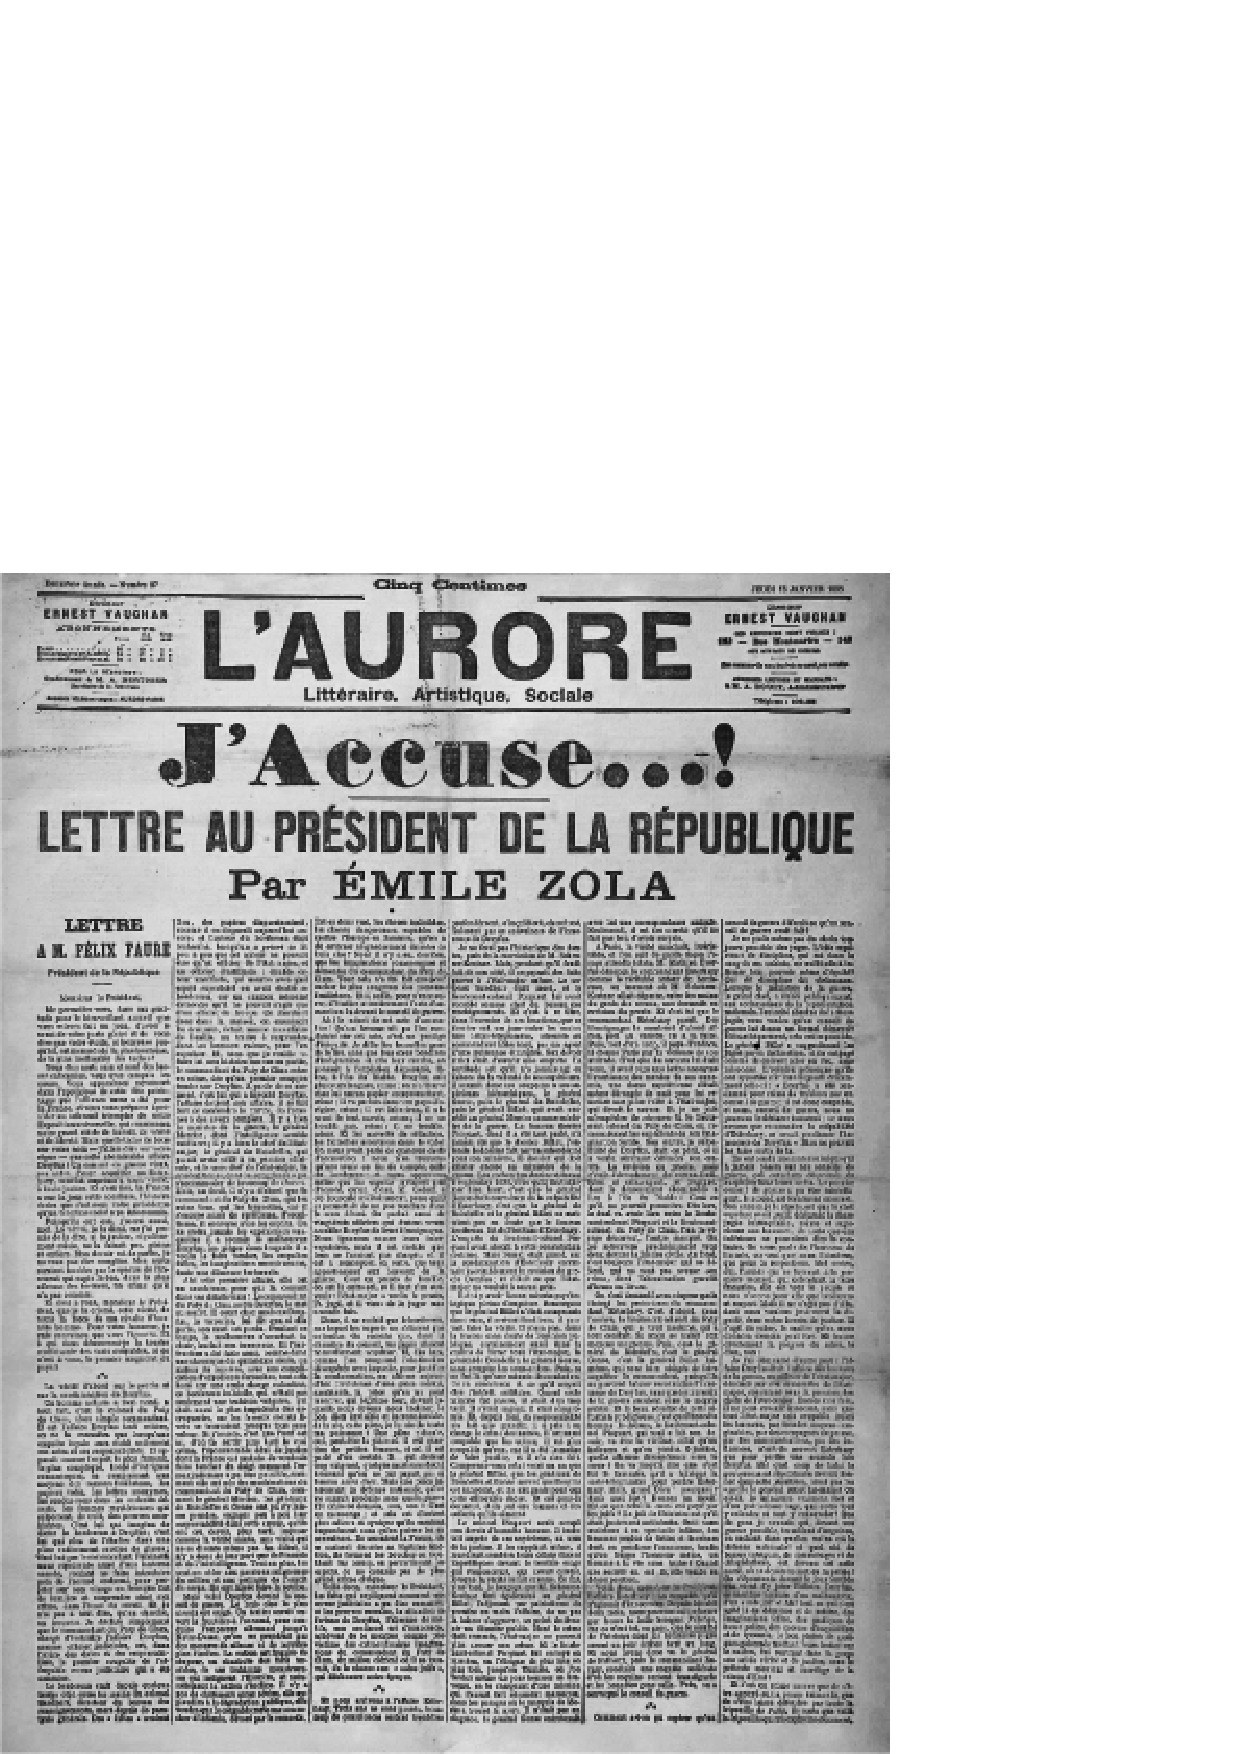
\includegraphics[width=7cm]{./img/00.pdf}
\legendas{\begin{center}Primeira página do jornal na qual figurou pela primeira
vez o artigo de Émile Zola, \textit{J'accuse!} [\textit{Eu
acuso!}].\end{center}}
\end{figure}

Depois de algum tempo o documento foi parar nas mãos do coronel
Sandherr, diretor do serviço de inteligência, que morreu de paralisia
geral. Então as coisas começaram a ``desaparecer'', papéis sumiram, como até hoje estão
sumindo; e foram atrás de saber quem era o autor do documento, e um
pré-requisito foi pouco a pouco se construindo: o culpado teria de
ser um oficial do Estado-Maior, e da artilharia: duplo erro
manifesto, que mostra a superficialidade com que o processo foi
tratado, pois um exame cuidadoso demonstra que o culpado
necessariamente precisa ser um oficial de tropa.

 Foi feita uma busca em domicílio, olharam os papéis, como se tudo fosse
um caso de família, uma tramoia a ser desvendada dentro dos escritórios
mesmo e então os culpados seriam expulsos. E, sem querer aqui contar
uma história já conhecida em parte, entra em cena o comandante du Paty
de Clam, quando as primeiras suspeitas começam a recair sobre Dreyfus.
Foi então que ele inventou um Dreyfus, o caso tornou-se o seu caso,
ele se esforçou para confundir o traidor e fazê-lo confessar tudo. Há
ainda o ministro da Guerra, general Mercier, cuja inteligência parece
medíocre; há o chefe do Estado-Maior, general Boisdeffre, que
aparenta ter cedido à sua paixão clerical, e o subchefe do
Estado-Maior, o general Gonse, cuja consciência se acomoda a quase
tudo. Mas, no fundo, não se trata de ninguém além do comandante du Paty
de Clam, que os guia a todos, que os hipnotiza, pois ele também se
ocupa do espiritismo, do ocultismo: ele conversa com os espíritos. É
impossível conceber as situações às quais ele submeteu o infeliz
Dreyfus, as armadilhas nas quais ele quis apanhá"-lo, as
investigações delirantes, as invenções montruosas, uma enorme demência
torturante.

Ah! Esse primeiro fato é um pesadelo para quem o conhece nos seus
verdadeiros detalhes! O comandante du Paty de Clam prende Dreyfus e o
coloca na solitária. Vai até a casa da senhora Dreyfus, amedronta"-a,
e diz que se ela contar alguma coisa para alguém seu
marido estará perdido. Durante esse tempo, o infeliz se desespera,
clamando inocência. E a instrução foi feita dessa forma, como se
fosse uma crônica do século \textsc{xv}, misteriosa, com expedientes cruéis,
tudo baseado exclusivamente em uma evidência infantil, esse documento
imbecil, que não passa de uma traição vulgar, a patifaria mais
grosseira, pois os famosos segredos transmitidos se revelaram todos sem
nenhum valor. Eu insisto porque é aqui que está a semente de onde
surgirá o verdadeiro crime, a espantosa recusa de justiça que torna a
França um lugar doente. Eu gostaria de entender como esse erro judicial
pôde ser possível, como ele surgiu das maquinações do comandante du
Paty de Clam; como o general Mercier e os generais de Boisdeffre e Gonse
puderam se deixar levar e torna-se pouco a pouco cúmplices desse
erro, que mais tarde acreditaram dever impor como uma verdade santa,
uma verdade indiscutível.  \textit{A priori}, só houve da parte deles
falta de cuidado e burrice. De mais a mais, sentimos que eles cederam
às paixões religiosas da comunidade e ao preconceito corporativista.
Permitiram que a estupidez acontecesse.

 Mas então Dreyfus se submete ao Conselho de Guerra. Exige-se o mais
absoluto sigilo. Mesmo que um traidor houvesse aberto a fronteira ao
inimigo para permitir que o imperador alemão tomasse Notre Dame, não
seriam tomadas precauções de sigilo e mistério tão severas. A nação
treme de espanto, um diz"-que"-diz de ocorrências terríveis, dessas
traições monstruosas que indignam a História; e naturalmente o país se
dobra. Não há punição que chegue, ele apoiará a degradação pública,
desejará que o culpado se enterre em um solo imutável de infâmia,
devorado pelo remorso. E, por isso, os fatos indizíveis, as coisas
perigosas capazes de incendiar a Europa e que por isso tiveram de ser
em sigilo soterrados serão verdadeiros? Não! Tudo não passou de fruto
da imaginação romanesca e desvairada do comandante du Paty de Clam. Tudo foi
feito apenas para esconder o mais estapafúrdio dos folhetins. Para que
isso fique claro, basta que o ato de acusação, lido diante do conselho
de guerra, seja analisado com um pouco de cuidado.

 Ah! A inutilidade desse ato de acusação! É um prodígio de iniquidade
que um homem tenha sido condenado por meio desse ato. Desafio todos os
homens corretos a lê-lo sem que seu coração se encha de indignação e
não grite de revolta, vendo o exagero da pena na distante Ilha do Diabo. 
Dreyfus domina vários idiomas: crime; não há um papel sequer em
sua casa que o comprometa: crime; de vez em quando ele retorna à sua
pátria: crime; trabalha muito, tem o cuidado de se informar sobre tudo:
crime; não perde a calma: crime; perde a calma: crime. E as
platitudes de redação, as assertivas formais no vazio! 
Falou-se em 14 itens de acusação: no final das contas, não encontramos mais
do que um, o tal documento; e já sabemos que nem com relação a ele os
especialistas estão de acordo; e que um deles, o sr. Gobert, foi
militarmente constrangido porque ousou chegar a uma conclusão diversa
daquela que se desejava. Falou-se ainda em 23 oficiais que
teriam arrasado Dreyfus em seus testemunhos. Nada sabemos do que
falaram, mas é fato que parte deles não o acusou; é obrigatório
observar, ainda, que todos pertenciam ao Ministério da Guerra. É um
processo interno, feito entre pares, e não se deve esquecer: 
o Estado-Maior queria o processo, levou a cabo o julgamento e termina de fazer outro.

 Portanto, nada mais que o documento, a respeito do qual os
especialistas não se entendem. Conta-se que, dentro da sala do
conselho, os juízes estavam na iminência de absolvê-lo. E, então,
para justificar a obstinação desesperada pela condenação, afirma-se
hoje que há um documento secreto, incontornável, um documento que não
se pode mostrar, que legitima tudo, diante do qual devemos nos
inclinar, o bom Deus invisível e incognoscível! Eu o recuso, recuso
esse documento, recuso-o com todas as minhas forças! Um documento
ridículo, sim, deve ser o documento em que se trata de umas mulherzinhas 
e se fala de um tal D\ldots que se transforma em figura
muito exigente: algum marido sem dúvida decepcionado por que não lhe
pagaram um bom preço por sua esposa. Mas esse documento, que interessa tanto à
defesa nacional, não poderia ser exibido sem que uma guerra fosse declarada amanhã, não, não! 
É mentira! E é de tal maneira odiosa e
cínica que essas pessoas mentem impunemente, sem que nada os convença.
Elas amotinam a França, escondem"-se atrás da sua legítima emoção,
fazem calar as bocas confundindo os corações, pervertendo os espíritos.
Não conheço crime cívico maior.

 Aqui está, portanto, senhor Presidente, os fatos que explicam como um
erro judiciário pôde ser cometido; e as provas morais, a situação do
destino de Dreyfus, a ausência de motivos, seu contínuo clamor de
inocência, exigem que eu o apresente como uma vítima da extraordinária
imaginação do comandante du Paty de Clam, do meio clerical em que ele
está, da perseguição aos “judeus sujos”, que desonra nossa época.

 E aqui chegamos ao caso Esterhazy. Três anos já se passaram, muitas
consciências permanecem profundamente confusas, inquietam"-se,
questionam e terminam se convencendo da inocência de Dreyfus.

 Não farei o histórico das dúvidas e da posterior certeza do sr. M.
Scheurer-Kestner. Mas, enquanto ele investigava por conta própria,
passavam-se fatos graves no próprio Estado-Maior. O coronel
Sandherr morre, e o tenente-coronel Picquart lhe sucede na chefia do
serviço de inteligência. E, por sua vez, no exercício de suas funções
foi que chegou às mãos desse último um telegrama, endereçado ao
comandante Esterhazy, remetido por um agente 
a serviço no exterior. Seu estrito dever era o de abrir uma sindicância. 
Fato é que ele nunca deixou de obedecer a seus superiores. Ele apresentou, pois, suas
suspeitas aos seus superiores hierárquicos, o general Gonse, depois o
general de Boisdeffre e, por fim, o general Billot, que ocupou o lugar
do general Mercier no Ministério da Guerra. O famoso dossiê Picquart,
de que tanto se fala, nunca foi nada além do que o dossiê Billot, um
dossiê feito por um subordinado para o seu ministro, dossiê que deve
ainda estar no Ministério da Guerra. As investigações duraram de maio a
setembro de 1896, e o que é preciso, dizer em alto e bom som é que o
general Gonse estava convencido da culpabilidade de Esterhazy e que o general
de Boisdeffre e o general Billot não tinham nenhuma dúvida de que o
autor do documento era Esterhazy. A investigação do tenente-coronel
Picquart tinha conduzido a essa constatação certeira. Mas o
constrangimento era grande, pois a condenação de Esterhazy acarretaria
necessariamente a revisão do processo Dreyfus; e isso é que o 
Estado-Maior queria evitar a qualquer custo.

 Deve ter havido um instante cheio de angústia psicológica. É fato que o
general Billot não estava comprometido com nada, ele tinha acabado de
saber de tudo, podia, portanto, dizer a verdade. Ele não ousou, temendo
sem dúvida a opinião pública, certamente também acreditando que
livraria todo o Estado-Maior, o general de Boisdeffre, o general
Gonse, sem falar dos inferiores. Depois, houve apenas um minuto de
combate entre a sua consciência e o que ele acreditava ser o interesse
militar. Quando esse minuto passou, já era muito tarde. Ele estava
engajado, já estava comprometido. E, desde então, sua responsabilidade
não para de crescer. Ele tomou para si o crime de outrem, é tão culpado
quanto os outros, é mais culpado que os outros, pois tinha a
oportunidade de fazer justiça, e não a fez. Veja isso! Faz um ano que o
general Billot, os generais de Boisdeffre e Gonse sabem que Dreyfus é
inocente, e guardam para si essa verdade aterradora! E dormem
tranquilos em casa, com suas esposas e filhos que os amam!

 O tenente-coronel Picquart estava cumprindo suas obrigações de homem
honesto. Insistia com seus superiores, em nome da justiça. Respondia,
dizia quanto suas decisões eram apolíticas, diante da terrível
tempestade que se construía, que se daria quando a verdade fosse
conhecida. Essa foi, mais tarde, a argumentação que M.
Scheurer-Kestner dirige igualmente ao general Billot, conclamando-o,
por patriotismo, a pegar o caso com as mãos, não deixá-lo mais se
agravar para evitar um desastre público. Não! O crime estava cometido,
o Estado-Maior não poderia mais evitar seu crime. E o
tenente-coronel Picquart foi enviado para o exterior, cada vez mais
distante, até a Tunísia, onde se quis até mesmo certa vez honrar sua
bravura, encarregando-o de uma missão que o teria seguramente
massacrado, em lugares em que o marquês de Mores encontrou a morte. Ele
não caiu em desgraça, o general Gonse manteve com ele uma
correspondência amigável. Apenas não era muito conveniente divulgar
alguns segredos.

 Em Paris, a verdade começava irresistivelmente a aparecer e sabia"-se
que em algum momento a tempestade explodiria. M.~Mathieu Dreyfus
denuncia o comandante Esterhazy como o verdadeiro autor do documento,
no mesmo momento em que M.~Scheurer-Kestner colocava, nas mãos do
Ministério da Justiça, um pedido de revisão do processo. E aqui aparece
o comandante Esterhazy. Testemunhas o descrevem de início
descontrolado, disposto a se suicidar ou fugir. Depois, de repente, 
cria coragem e assusta Paris pela violência de sua atitude.  É que
tinha chegado ajuda, ele havia recebido uma carta anônima advertindo"-o
das manobras de seus inimigos, uma dama misteriosa chegou mesmo a se
abalar durante a noite para roubar do Estado-Maior um documento
que o salvaria. E aqui eu não posso deixar de lembrar a
imaginação fértil do comandante du Paty de Clam. Sua obra, a
culpabilidade de Dreyfus, estava em perigo, e ele quis seguramente
defender a própria criação. A revisão do processo, seria esse o
desfecho do extravagante e trágico folhetim, cujo abominável
desenlace realizou"-se na Ilha do Diabo! Isso ele não podia permitir.
Então, o duelo ocorrerá entre o tenente-coronel Picquart e o
comandante du Paty de Clam, um de cara aberta, o outro mascarado. 
Nós os reencontraremos em breve, diante da justiça civil. No fundo, é sempre o
Estado-Maior que se defende, que não quer admitir seu crime, cuja abominação cresce a cada hora.

Com espanto, perguntou-se quem eram os protetores do comandante
Esterhazy. Em primeiro lugar, na surdina, o comandante du Paty
de Clam, que maquinou e coordenou a coisa toda. Ele foi traído 
pelos seus próprios métodos bizarros. Depois, é o general de Boisdeffre, o
general Gonse, e o próprio general Billot, que são obrigados a absolver
o comandante, já que não podem deixar que a inocência de
Dreyfus seja reconhecida sem que o Ministério da Guerra caia em descrédito. E o
fantástico resultado dessa prodigiosa situação é que o honesto
tenente-coronel Picquart, que apenas cumpriu seu dever, será ele
a vítima, o ridicularizado e o punido. Ah!, justiça, que terrível
desespero rasga o coração! Chega-se ao cúmulo de dizer que ele é o
falsificador, que fabricou o telegrama para incriminar Esterhazy. Mas, ó
Deus! Por quê? Com que razão? Dai-me um motivo. Ele também foi pago
pelos judeus? O mais engraçado é que ele é justamente o anti-semita!
Sim! Assistimos a esse espetáculo infame, homens perdidos em dívidas e
crimes que se proclamam inocentes, enquanto se mancha a honra de um
homem de vida irrepreensível. Quando uma sociedade chega a esse ponto,
está desintegrada.

 Eis, portanto, senhor Presidente, o caso Esterhazy: um culpado que era preciso inocentar.
Retroagindo dois meses, podemos acompanhar hora
por hora esse admirável serviço. Vou abreviar, pois aqui não trago nada mais que um
resumo da história, cujas páginas vibrantes serão um dia escritas na íntegra.

E, então, vimos o general de Pellieux, depois o comandante
Ravary, conduzir uma investigação criminosa em que os canalhas foram
purificados, e os honestos, manchados. Logo depois, o Conselho de Guerra foi
convocado.

 Como se pode esperar que um Conselho de Guerra corrija o erro de outro
Conselho de Guerra?

E nem estou me referindo aqui à escolha dos juízes. A ideia superior de
disciplina, que corre no sangue desses soldados, não bastaria por si só
para invalidar sua capacidade de julgar imparcialmente? Quem fala disciplina, fala obediência. 
Quando o ministro da Guerra, a principal
autoridade, estabeleceu publicamente, sob os aplausos da representação nacional, a
autoridade do julgamento, não se pode esperar que um Conselho de Guerra
o desminta. Hierarquicamente, é impossível. O general Billot
influenciou os juízes com a sua declaração, e eles a julgaram como se devessem partir para o ataque,
sem refletir. A opinião preconcebida,
que levaram para o julgamento, é evidentemente essa: “Dreyfus foi
condenado por traição por um Conselho de Guerra, é, portanto, culpado;
e nós, o Conselho de Guerra, não podemos declará-lo inocente, pois
 sabemos que reconhecer a culpa de Esterhazy é proclamar a
inocência de Dreyfus”. Nada os demoveria dessa ideia.

 Proclamaram uma sentença iníqua, que pesará para sempre sobre
os nossos conselhos de guerra e que manchará de suspeita daqui em diante todas as suas
decisões. O primeiro Conselho de Guerra não foi inteligente; mas o segundo é
forçosamente criminoso. Sua desculpa, repito, é que a autoridade
principal já tinha decidido, declarando inatacável o julgamento
anterior, santo e superior aos homens, de modo que os inferiores não
podiam dizer o contrário. Falam"-nos da honra do exército, querem
que nós o amemos e o respeitemos. Ah!, claro, o exército que se
erguerá diante da primeira ameaça, que defenderá o território
francês, ele é o povo, e não sentimos por ele nada além de ternura e
respeito. Mas não se trata dele, de quem, em nossa necessidade de justiça, desejamos justamente a dignidade. 
Trata"-se aqui do sabre, o senhor que, quem sabe, nos darão amanhã. Mas beijar com devoção seu punho, ó deus, isso não! 

Já o demonstrei: o caso Dreyfus foi o caso do Ministério da Guerra;
um oficial do Estado-Maior, denunciado por seus colegas do
Estado-Maior, condenado sob a pressão dos chefes do Estado-Maior.
E mais uma vez: ele não pode ser inocentado sem que todo o
Estado-Maior seja culpado. Também os ministérios, por todos os meios imagináveis,
com campanhas nos jornais, com comunicados e tráfico de
influência, só cobriram Esterhazy para culpar Dreyfus uma segunda vez. 
Ah! o governo republicano deveria pôr no olho da rua esse bando de jesuítas, 
como o próprio general Billot os chama!  

Onde está o ministério verdadeiramente forte, de um patriotismo sábio, 
que terá a coragem de tudo renovar e recriar? Quanta gente
não conheço que, diante de uma possível guerra, treme de angústia
sabendo em que mãos está a defesa nacional? E a que ninho de
baixarias, fofocas e esbanjamentos está entregue esse lugar sagrado,
onde se decide o futuro da pátria? Assusta o que o caso Dreyfus acabou
revelando, esse sacrifício humano de um infeliz, de um “judeu porco”!
Ah!, que agitação de demência e imbecilidade, de
imaginações estúpidas, de práticas de políticas mesquinhas, de costumes
inquisitoriais e tirânicos, a satisfação de alguns oficiais agaloados esmagando
a nação com suas botas, enfiando goela abaixo seu grito de verdade e justiça,
sob o pretexto mentiroso e sacrílego da razão de estado!

 E é um crime ainda terem se apoiado na imprensa imunda, terem se deixado
defender por toda a canalha de Paris, 
de modo que é essa canalha que triunfa insolenemente, 
diante da derrota do direito e da simples probidade.  É um crime terem acusado de perturbar a 
França aqueles que a querem generosa, na vanguarda das nações livres e justas, quando tramaram
eles próprios a impudente conspiração para impor o erro ao mundo inteiro.  
É um crime confundir a opinião pública, utilizar para uma sentença fatal
essa opinião pública que foi corrompida até o delírio. É um crime
envenenar os pequenos e humildes, exasperar as paixões de reação e de
intolerância, abrigando-se atrás de um odioso anti-semitismo, de que a grande
França liberal dos direitos do homem sucumbirá, se não for curada.
É um crime explorar o patriotismo para as obras do ódio; é um crime, por
fim, fazer do sabre o deus moderno, quando toda a ciência humana está a
serviço da obra iminente da verdade e da justiça.

 Essa verdade, essa justiça, que tão apaixonadamente desejamos, que
aflição vê"-las assim esbofeteadas, mais desprezadas e mais
obscurecidas! Desconfio do desmoronamento que se deu na alma de
Scheurer-Kestner, e acredito que ele acabará sentindo remorso, o de
não ter agido revolucionariamente no dia da interpelação no Senado,
revelando o que sabia, para pôr tudo abaixo. Foi o grande homem de bem
da história, o homem de vida leal, acreditou que a verdade se
bastaria a si própria, sobretudo quando ela lhe aparecia clara como a luz do dia.  
De que valeria todo o transtorno, se logo o sol a tudo esclareceria?
E foi por essa serenidade confiante que foi tão cruelmente punido. O mesmo
para o tenente-coronel Picquart, que, por um sentimento de grande
dignidade, não quis publicar as cartas do general Gonse. Esses
escrúpulos o tornam ainda mais honrado quando sabemos que, enquanto ele
se mantinha respeitoso na disciplina, seus superiores o faziam
cobrir-se de lama, instruindo eles mesmos o processo, da maneira mais
inesperada e ultrajante. Há duas vítimas, dois homens corajosos, dois
corações simples, que se entregaram a Deus, enquanto o Diabo se
movimentava. E até mesmo se viu, da parte do tenente-coronel Picquart, essa
ignomínia: um tribunal francês, depois de ter permitido que o promotor atacasse 
publicamente uma testemunha, acusando-a de todos os
crimes, passar à audiência secreta justamente quando a testemunha começou a se explicar e
a se defender. Afirmo ser este mais um crime, um crime que provocará a indignação
da consciência universal. Decididamente, nossos tribunais
militares têm uma ideia muito particular de justiça.

 Essa é, pois, a simples verdade, senhor Presidente, e ela é
assustadora, e marcará sua presidência como uma mancha. Desconfio que o 
senhor não pode fazer nada esse respeito, que é prisioneiro da
Constituição e de seus assessores. Mas tem ainda assim um dever como homem, 
no qual pensa, e que cumprirá. Não que eu duvide, aliás, nem um pouco, que a 
verdade triunfará. Repito"-o, e com uma certeza ainda mais veemente: 
a verdade está a caminho e ninguém a deterá. As coisas estão apenas 
começando, pois apenas agora os fatos estão claros: de um lado,
os culpados que não querem que a justiça se faça; de outro, os honestos
que darão sua vida para que ela se faça. Já o disse antes, e vou
repeti"-lo aqui: quando a verdade fica soterrada, ela toma corpo, e
ganha tal força explosiva que, quando explode, leva tudo consigo.
Veremos se o que acaba de ser preparado não será mais tarde o mais retumbante dos desastres.

 Mas esta carta já vai longe, senhor Presidente, e é hora de concluí-la.

 Acuso o comandante du Paty de Clam de ter sido o criador
diabólico do erro judicial, inconscientemente, quero crer, e de ter
saído em defesa de sua obra nefasta, durante três anos, por maquinações
as mais estapafúrdias e as mais culposas.

Acuso o general Mercier de ter se tornado cúmplice, ainda que por
fraqueza de caráter, de uma das maiores iniquidades do século.

Acuso o general Billot de ter tido entre as mãos as provas
indubitáveis da inocência de Dreyfus e de tê-las ocultado,
tornando-se, pois, culpado de crime de lesa-humanidade e lesa"-justiça,
por motivos políticos e para livrar um Estado-Maior comprometido.

Acuso o general de Boisdeffre e o general Gonse de tornarem-se
cúmplices do mesmo crime, um sem dúvida por paixão clerical, o outro
por esse corporativismo que faz do Ministério da Guerra uma arca santa
inatacável.

Acuso o general de Pellieux e o comandante Ravary de terem feito uma
investigação criminosa, um inquérito da mais monstruosa parcialidade
e do qual temos, no relatório do segundo, um monumento perene da mais ingênua audácia.

Acuso os três especialistas em grafologia, os senhores Belhomme,
Varinard e Couard de terem emitido pareceres mentirosos e fraudulentos, a
menos que um laudo médico os declare tomados por alguma patologia da
vista e do juízo.

Acuso o Ministério da Guerra de ter promovido na imprensa,
particularmente no \textit{L'Éclair} e no \textit{L'Écho de Paris}, uma
campanha abominável, para manipular a opinião pública e acobertar sua falha.

Acuso por fim o primeiro Conselho de Guerra de ter violado o direito,
condenando um acusado com base em um documento secreto, e acuso o segundo
Conselho de Guerra de ter encoberto essa ilegalidade, por ter recebido
ordens, cometendo por sua vez o crime jurídico de absolver conscientemente um culpado.

Fazendo essas acusações, não ignoro enquadrar"-me nos artigos 30
e 31 da lei de imprensa de 29 de julho de 1881, que pune os delitos de
difamação. E é voluntariamente que eu me exponho.

Quanto às pessoas que eu acuso, não as conheço, nunca as vi, não
nutro por elas nem rancor nem ódio. Não passam para mim de
entidades, de espíritos da malevolência social. O ato que aqui realizo
não é nada além de uma ação revolucionária para apressar a explosão de
verdade e justiça.

Não tenho mais que uma paixão, uma paixão pela verdade, em nome da humanidade que
tanto sofreu e que tem direito à felicidade. Meu protesto inflamado
nada mais é que o grito da minha alma. Que ousem portanto levar"-me perante ao tribunal do júri
e que o inquérito se dê à luz do dia! 

É o que espero.

Receba, senhor Presidente, minhas manifestações de mais profundo
respeito.

\part{o processo do capitão dreyfus}

\chapter[O processo do capitão Dreyfus,\\por Rui Barbosa]{o processo\break do capitão dreyfus\subtitulo{por Rui Barbosa}}
\hedramarkboth{O processo do capitão Dreyfus}{Rui Barbosa}

\begin{flushright}
(Londres, 7 de janeiro de 1895.) 
\end{flushright}

Eis aí um fato, de expressão quase trágica, sobre o qual se acaba de
exercer distintamente a consciência dos dois povos que a Mancha separa:
um, na maneira de resolvê-lo; o outro, na de considerá-lo.
Decompostas através dele, como dois feixes diferentes de luz coados
pelo mesmo prisma, destacam-se em matizes característicos certas
qualidades de ordem moral, predominantes no espírito e na história das
duas grandes nações.

Tudo quanto ressumbra das causas que geraram a terrível sentença,
resume-se na frase interrompida, em que Madame Démange, ao abrir da
audiência, declarou que a acusação inteira assentava exclusivamente em
um documento contestado. A esta revelação do advogado, o oficial
presidente lhe cortou a palavra, votou-se o \textit{huis-clos}, 
e a instância imergiu no mistério, cujo termo é a condenação do acusado a penas de
irresgatável infâmia.

Não me cabe descrever a cerimônia atroz da degradação militar, prelúdio
feroz da expiação sobre-humana, que se abriu ontem para o malfadado.
Essa cruel solenidade horrorizou a Europa. Antes de se separar
irremissivelmente da Pátria, amaldiçoado pelos seus conterrâneos, para
ir agonizar, sob o indelével ferrete, em remoto presídio penal, esse
infeliz passou pelos tratos do mais tremendo suplício conhecido na
história das torturas morais. O formidável espetáculo fora preparado
com todos os requintes da encenação regulamentar. Quando o condenado
entrou no quadrângulo da Escola Militar, as insígnias, que ainda lhe
sobressaíam na farda, já não figuravam ali senão por artifício
convencional, como outros tantos estigmas no peito e na fronte daquele
homem. O alfaiate substituíra de véspera as costuras por alinhavos; o
cutileiro partira e ressoldara a espada, que no outro dia se devia
quebrar publicamente diante das tropas. A lenta e implacável pragmática
esgotou no flagelado o cálix das afrontas possíveis. Se entre elas não
figura o esbofeteamento, dir-se-ia que não é senão para poupar à
mão do executor o vilipêndio do contato com o rosto do réprobo. Desde
o \textit{képi} até as listas vermelhas das calças, um a um, lhe caíram aos pés,
arrancados por um subalterno, os emblemas da dignidade militar.
Ficaram-no envolvendo apenas os restos negros e rotos da farda,
imagem do luto pela honra que acabava de despir. Nesse miserável
extremo, ainda lhe coube a penitência de transpor as filas do quadrado;
e, entregue então à polícia civil, submetido, como os criminosos
comuns, à medição antropológica, passou das mãos dos seus camaradas às
dos gendarmes, para acabar os dias em Nova Caledônia, entre a escória
dos criminosos, onde a família irá respirar com ele o ar dos galés.

Qualquer que fosse o crime daquele desgraçado, a rebuscada e caprichosa
desumanidade dessa punição revolta profundamente o  
sentimento contemporâneo. Aqui o efeito foi de indignação e espanto. A
repugnância ao escândalo por pouco se não transmudou em misericórdia e
simpatia pelo aflito, ``A cerimônia da
degradação'', escreve o sr. de Blowitz em um dos seus
telegramas ao \textit{Times}, ``apresenta hoje em dia um espetáculo
de aspecto bárbaro, do qual nenhuma lição se pode colher. É deplorável
que se não pudesse pronunciar a pena de morte''.

A \textit{Pall Mall Gazette}, uma das folhas inglesas que mais reserva guardaram
no tocante ao processo Dreyfus, soltou esta tarde os diques ao seu
\textit{humour} e à sua severidade nestas palavras:

\begin{hedraquote}
Não há muito que a Europa metia à bulha o imperador da China pelo seu
sistema obsoletamente bárbaro de punir arrancando botões ao acusado.
Contudo, o contágio já se comunicou à França. Custa a
perceber o proveito da repulsiva cena celebrada sábado na praça da
Escola Militar. A degradação simbólica, nas leis militares, é uma
relíquia da Média Idade, em que a investidura se operava também por
um ritual solene. Compreendemos o clamor pela execução de espiões e
traidores. Compreenderíamos, até, como recurso disciplinar, a eficácia
e o valor de um aparato como esse, quando levado a efeito no campo de
batalha. Mas, devemos confessá-lo, os pormenores da degradação,
concebidos e postos por obra a sangue-frio, meses após a perpetração
do alegado crime e semanas depois da sentença proferida contra o
infeliz, deixam-nos a impressão de uma penalidade quase materialmente
idêntica à tortura.
\end{hedraquote}

Dilacerante, como é, todavia, essa expiação no seu cortejo de
circunstâncias terríveis, não conseguiu moderar, em França, o espasmo
de ódio insaciável, que agita contra o acusado todas as classes da
população. ``Até agora'', observa o correspondente do 
\textit{Daily News}, ``não se imaginava a comoção
de Paris, quando, há um século, ao reboar o grito de perigo da Pátria,
o rei e a rainha foram enviados ao cadafalso como cúmplices da invasão
estrangeira''. Mas as cerimônias da guilhotina nem sempre
acabam entre bravos e palmas, como a execução do assassino de Carnot.
Entre os espectadores do patíbulo há, muitas vezes, corações tocados de
compaixão e olhos úmidos de lágrimas. Na turba que cercava de longe o
suplício de Dreyfus, só havia lampejos e acentos de ira. Tão miseranda é
a sua sorte que a polícia, ao que se diz, terá de adotar precauções,
para lhe defender a vida contra a indignação patriótica dos
calcetas. E, segundo o \textit{Figaro}, quando o ex-oficial, saciado de
opróbrio, ao passar pelos oficiais da reserva, renovou o seu protesto
insistente de inocência, um deles cuspiu-lhe à face o epíteto de
``Judas''.

\begin{hedraquote}
Este episódio [telegrafa o correspondente do \textit{Times}] recorda-me o que
se deu, no ano de 1871, em Bordeaux, quando a Assembleia ali
trabalhava. O serviço de sentinelas fora confiado à Guarda Nacional,
que aderira à República, e tinha em conta de reacionária a Assembleia.
Uma vez, quando Thiers descia as escadas do teatro, onde ela
funcionava, um guarda nacional gritou: \textit{Vive la république!} Thiers, com
o olhar chispeante, caminhou para o soldado, sacudiu-o pelo braço, e,
com o agudo peculiar de sua voz, ainda mais timbrada pela paixão, lhe
bradou ao ouvido: \textit{On ne parle pas sous les armes.}
Desconfio que ele teria dito o mesmo a este oficial da reserva, futuro guarda nacional.
\end{hedraquote}

Que faculdade sobre-humana deu àquele homem energia bastante, para
sobreviver às emoções incomportáveis dessa provação? A não se tratar de
um miserável, bronzeado na fronte, calejado no coração pela prática
habitual dos vícios que emasculam o caráter, e saturam de impudor os
mais baixos vilões, só duas forças seriam capazes de forrar uma alma
contra a abjeção incomparável daquela queda, contra o desespero
inaudito daquele destino: a insânia, ou a inocência. Ora, Dreyfus não
tinha no seu passado uma nódoa, um traço duvidoso. Quinze anos de
serviços imaculados e a alta posição de confiança, que ocupava no mais
delicado ramo da administração da guerra, definem-lhe a fé de ofício.
A superabundância dos seus recursos, a opulência de sua família, a
simplicidade dos seus hábitos, a sua aversão ao jogo, a concentração
exclusiva da sua vida particular nas afeições domésticas excluem a
suspeita das seduções tenebrosas, que são frequentemente a explicação
obscura dessas catástrofes da honra. De onde viria, pois, a tentação
inexplicável, que instantaneamente prostituiu aquele ornamento da sua
classe, aquela nobre esperança dos seus concidadãos?

Narram as testemunhas atentas do suplício que o executado não
empalideceu nunca. Os passos não lhe vacilaram. Não lhe tremeu a voz. A
cabeça esteve-lhe sempre erecta. Ao ver, de manhã, preparada a sua
farda para a cerimônia, ``Capitão'', disse
ele ao oficial presente, ``estais sendo instrumento da
maior injustiça deste século''. Quando, ao empuxão do
executor, o \textit{képi} lhe desceu sobre os olhos a mão levantou-se-lhe
como invocação de um inocente: ``Por minha mulher e meus
filhos'', exclamou, ``juro que sou inocente.
Viva a França!'' Aos apupos de um grupo de oficiais,
``com admirável império sobre si mesmo'', diz
um jornalista, respondeu serenamente: ``Feri, mas não
insulteis. Eu sou inocente''. E, ainda ao sair, no momento
em que os gendarmes lhe punham algemas, teve forças, para dizer aos
seus camaradas do 59 de Infantaria: ``Crede-me,
senhores, sou um mártir!''

A insistência desse protesto, com as circunstâncias que o distinguem,
precedem, e circundam, não tem analogia na crônica das hipocrisias do
crime.~Sua repercussão no jornalismo inglês, alheio às alucinações
locais, sóbrio, como se sabe, em pontos de sentimentalismo, mas
inclinado à retidão própria dos costumes jurídicos deste país, foi
vasta e profunda.

A \textit{Pall Mall Gazette} enuncia-se assim:

\begin{hedraquote}
Segundo todas as informações, o capitão Dreyfus sofreu a provação mais
dilaceradora, a que se podia expor um homem, de cuja sensibilidade
moral ainda restasse alguma coisa, com um estoicismo antes conciliável
com o sentimento da inocência do que com a consciência do crime.
\end{hedraquote}

E, depois de considerar nas antecedências honrosas do condenado,
conclui: ``A ser assim, Dreyfus será um inocente, ou um louco.''

O \textit{Daily Graphic}, que ainda se não pronunciara a favor dele, remata hoje
com estas ponderações:

\begin{hedraquote}
As dúvidas existentes e francamente exprimidas fora da França na questão
da criminalidade ou inocência de Dreyfus não sofrerão quebra, por
certo, em presença da singular fortaleza com que o condenado padeceu o
medonho castigo. A sua firme protestação de inculpabilidade tende
naturalmente a suscitar a crença de algum erro cometido contra ele.
\end{hedraquote}

Mas entre franceses não é lícito sequer pôr em dúvida o crime de
Dreyfus: ``Quem quer que deixasse transparecer, a esse
respeito, a menor incerteza, ou denotasse o mais leve sentimento de
comiseração, seria encarado com o mesmo horror e o mesmo ódio que o
próprio traidor.'' Pleno arbítrio de negar a Deus, aluir a
propriedade, santificar a comuna, divinizar Marat; mas obrigação
estrita e universal de teimar e bater pé em como Dreyfus é o mais
desprezível dos malfeitores. ``Nisto se afincou o público
desde o primeiro dia'', escreve um correspondente inglês.
``Criminoso de quê, esse criminoso? Ninguém o sabia: e,
até hoje, ninguém, dentre o público, o sabe. Todavia, a existência da
traição passou em julgado como fato indisputável.''

Onde o corpo de delito? Onde a identificação entre o seu autor e o
acusado? Ninguém seria capaz de mostrá-lo. Ninguém viu o processo.
Ninguém tem notícia de documentos, ou depoimentos. Fala-se em um
papel, cuja letra se atribui ao condenado. Mas o que a esse propósito
se conhece, por indiscrições publicadas no \textit{Figaro}, é que, de cinco
peritos ouvidos sobre o caráter da letra nesse escrito anônimo, se três
reconhecem a de Dreyfus, dois sustentam o contrário.

Essa multidão espumante, que cercava, ameaçadora, a Escola Militar,
bramindo insultos, assuadas e vozes de morte, --- que mais era,
portanto, afinal, do que uma força violenta e cega, como os movimentos
inconscientes da natureza física? Pela minha parte, não conheço
excessos mais odiosos do que essas orgias públicas da massa
irresponsável. Nada seria menos estimável, neste mundo, que a
democracia, se a democracia fosse isto. Esses escândalos representam o
pior desserviço à dignidade do povo, e constituem o mais especioso
argumento contra a sua autoridade. Não é sob tais formas que ele se há
de mostrar digno da soberania, cujo cetro as tendências da nossa época
lhe reconhecem. Se o número não souber dar razão dos seus atos, se as
maiorias não se legitimarem pela inteligência e pela justiça, o Governo
popular não será menos aviltante que o dos autocratas. Nem a invocação
da Pátria imprime a tais desvios fisionomia menos antipática. Mal
honram a Pátria as contorsões de um patriotismo histérico, que vive a
se superexcitar com a obsessão de traições, que julga de oitiva,
fulmina por palpites, e instiga os magistrados a prevaricar,
antepondo a popularidade à justiça.

Aqui, onde não chega o revérbero ardente do braseiro francês, ninguém
compreende o encarniçamento da imprensa daquele país sobre o cadáver
moral de Dreyfus. O Governo excluiu da cerimônia os jornalistas
estrangeiros, sob uma razão de decência. O pudor da França queria
encerrar no círculo doméstico o aparato da ignomínia de um homem, que
vestia o glorioso uniforme do Exército francês. Entretanto, no dia
imediato à execução, parecia ter-se posto a prêmio entre os jornais,
como tema de concurso literário, a descrição do espetáculo, sobre cuja
humilhante crueldade se tinha querido baixar o véu da vergonha, o mesmo
véu, que, ao menos por coerência, diz o \textit{Standard}, devia ter coberto a
execução de uma sentença, cuja gestação se incubou às ocultas.

Não contentes, os diretores morais da opinião, naquela grande metrópole
de tantas cruzadas humanitárias e liberais, encetaram uma campanha, a
que se diz vai ceder o Governo, para se aditar aos sítios de degredo a
Guiana Francesa, que oferece aos irritados pela benignidade da
condenação de Dreyfus a segurança de uma polícia mais eficaz e um clima
ainda mais funesto ao homem do que o da Nova Caledônia. Custa a
compreender que interesse nacional possa haver, deveras, para a França
em acumular sofrimentos sobre os restos de vida sobrenadantes àquele
naufrágio. Nessa extrema descaridade, parece haver alguma coisa da
mutilação após o sacrifício, que, em certos estados, bárbaros,
assinalava os costumes penais, e revelar-se a \textit{bête humaine}, acordando
inesperadamente no homem civilizado. Pois em verdade ainda haveria
agonias que espremer daquela agonia? Para a lição moral, assim como
para o efeito expiatório, a medida ainda teria muito que encher?

Como quer que seja, votar uma lei, para agravar a miséria de um
condenado, seria singular novidade na história penal destes tempos.
Nessa medida, adotada especial, senão expressamente, para
sobrecarregar as consequências de uma sentença já proferida, ferindo
um homem já esmagado, há uma intenção de vindita individual, um caráter
de rancor, um elemento retroativo, que as noções de direito cristão não
tolerariam. Não importa que seja apenas trocar degredo por degredo. Se
a nova localidade se elege, por ser mais áspera, mais inóspita, menos
habitável do que as contempladas na lei sob que se proferiu o julgado,
a alteração projetada seria, em substância, uma verdadeira revisão de
sentenças por ato legislativo, isto é, um mal dissimulado exemplo dessa
retroatividade penal, que todas as legislações contemporâneas
estigmatizam.

Se os oficiais que compunham o Conselho de Guerra dispusessem, na
hipótese, da pena de morte, certamente, a meu ver, não hesitariam em
pronunciá-la. Essa decisão, mais clemente e mais heroica a um tempo,
encerraria, ainda, para a classe a que pertencia o degradado, a
vantagem de poupar-lhe, com a eliminação imediata dessa existência
aviltada, o reflexo inevitável de vergonha destingido sobre os seus
antigos companheiros de armas. Só um obstáculo insuperável na letra da
lei poderia deter a mão aos juízes fardados, em cujo espírito a
indignação e a piedade, de mãos dadas, deviam pleitear pela pena capital.

O tribunal recuou, com efeito, ante disposições legislativas na sua
opinião inelutáveis. O art.~76 do Código Penal consignava a morte como
a pena reservada aos crimes da natureza do imputado a Dreyfus. Mas a
Constituição de 1848 aboliu a pena de morte nos delitos políticos,
entre os quais se incluía a traição militar, e a lei de 8 de junho de
1850 fixou, para esses casos, o degredo com prisão perpétua numa
fortaleza, acrescentando que as pessoas incursas nessa 
cominação desfrutariam a liberdade compatível com a segurança necessária à
custódia dos condenados.

Não me cabe apreciar o acerto, ou desacerto, do direito francês neste
ponto. Computando a traição militar entre os delitos políticos, ele
obedeceu à lógica de uma filantropia, cuja influência se assinalou no
Brasil republicano por um espécimen curioso, na extinção absoluta da
pena de morte por estatuto constitucional, com reserva apenas das
disposições militares em tempo de guerra. Todos aliás conhecem o valor
dessa barreira moral em certos países. Na França, porém, os juízes de
Dreyfus, apesar de homens de espada, a consideraram inviolável. Se
houvessem de pronunciar-se como legisladores, o seu voto seria
provavelmente diverso. Aquele que tachar de excessiva a pena de fuzil,
para o crime de que se acusa Dreyfus, não poderia admiti-la para
outro. Se há delito equiparável ao parricídio, é esse, felizmente não
menos raro do que o seu congênere. O oficial que entregou ao inimigo os
planos de defesa da Pátria, emparelha com o que vende ao inimigo a vida
dos seus camaradas. O opróbrio dessa inconfidência suprema equivale ao
da traição no campo. Um soldado, um cidadão não pode perpetrar atentado
mais negro. Não há militar, não haveria talvez estadista, que não lhe
cominasse resolutamente a última pena.

Uma coisa, porém, é fazer a lei; outra, executá-la. E os julgadores de
Dreyfus, unânimes em condená-lo, acordaram com a mesma unanimidade no
respeito ao seu papel de aplicadores da vontade escrita do legislador.

Na dignidade com que desempenharam essa grave magistratura, no Império,
que, a bem dela, exerceram sobre os seus próprios sentimentos e as
paixões dos seus compatriotas, aqueles sete oficiais deram à opinião
versátil e irritadiça do país um exemplo virtuoso. A França, porém, não
se satisfez com a sentença. No sentir, porque assim digamos, unânime de
Paris, Dreyfus devia ter sido condenado à morte. Essa foi a voz das
ruas, a da imprensa e a da tribuna. Os radicais trovejaram tempestades
contra o Governo e a situação social. O Parlamento incendiou-se em
uma cena de escândalo. O próprio elemento moderado teve que render o
seu preito à força da corrente, propondo às Câmaras, por órgão do
Governo, a cominação da pena extrema à espionagem em tempo de paz; como
se a precipitação remediasse o caso julgado, ou se as reformas semeadas
pelos furacões políticos na região do direito penal pudessem lançar
raízes na consciência dos povos, e levantar-lhes a moralidade.

O ``povo soberano'', os partidos e governos,
entre as nações sem disciplina jurídica, estão sempre inclinados a
reagir contra as instituições que se não dobram aos impulsos das
maiorias e às exigências das ditaduras. A lei foi instituída exatamente
para resistir a esses dois perigos, com um ponto de estabilidade
superior aos caprichos e às flutuações da onda humana. Os magistrados
foram postos especialmente para assegurar à lei um domínio tanto
mais estrito, quanto mais extraordinárias forem as situações, mais
formidáveis a soma de interesses e a força do poder alistados contra
ela. Mas há nações, que a não toleram senão como instrumento
``dos tempos ordinários''; e, se encontram
nela obstáculo às suas preocupações, ou às suas fraquezas, vão buscar a
salvação pública nos sofismas da conveniência mais flexível, a cuja
sombra os impulsos instintivos da multidão, ou as aventuras
irresponsáveis da autoridade se legitimam sempre em nome da
necessidade, da moral, ou do patriotismo.

Não há mais odiosa iniquidade, alegam, do que passar pelas armas o
conscrito, cuja mão, sob o frenesi de um desvario momentâneo, se
levantou contra o seu superior, e poupar a vida ao oficial, que
refletida e interessadamente, ``atraiçoa a sua Pátria,
isto é, alia-se, contra ela, ao estrangeiro''. Assim
discorre a dialética, e assim raciocina o francês. Porque o francês não
adverte em que a lei é a lei com todas as suas insuficiências, todas as
suas desigualdades, todos os seus ilogismos, e em que a observância
dela é o caminho para a sua reforma, único remédio real aos seus
defeitos, menos funestos, em todo caso, do que o arbítrio da razão
humana, encarnada no número, no poder ou na força.

Certo, responde o inglês, no seu ponto de vista, que acabo de antecipar;
certo o crime de Dreyfus, é tamanho, quanto o do pobre soldado, senão
maior, muito maior: ``Mas'' (e aqui deixo
falar um dos mais altos inspiradores da opinião do Reino Unido),

\begin{hedraquote}
o caso é que a lei fixa a morte como a cominação adequada, numa espécie,
não na outra; ``e os exércitos não se mantêm senão pela
mais rígida aderência a leis inflexíveis''. Se o capitão
Dreyfus fosse fuzilado, nenhum oficial mais nunca se sentiria em
segurança; porque, de futuro, qualquer outra lei, que tocasse a
oficiais, poderia ser conculcada por uma explosão do sentimento
público. Assim, por exemplo, a que legitimasse a repressão militar de
movimentos sediciosos. Se a lei favorece em demasia os traidores, é
modificarem a lei. A Câmara francesa trata agora de converter em delito
de pena capital a traição, ainda quando inspirada por motivos
políticos. Pela nossa parte, não temos que objetar. Fuzilar, porém, o
capitão Dreyfus, em virtude de uma disposição retroativa, seria
extinguir esse sentimento de confiança na seriedade da lei,
``tão essencial à disciplina quanto a própria severidade''.
\end{hedraquote}

Estas palavras são do \textit{Spectator}, que representa, na Inglaterra, a mais
fina flor da cultura jornalística e, ao mesmo tempo, o equilíbrio mais
exato entre as opiniões moderadas.

A tendência, não sei se diga francesa, se latina, a condenar por
impressões, a antecipar as sentenças, a se substituir aos juízes, e a
ditar arestos aos tribunais tomou, neste ominoso episódio, feições
dignas de estudo no seu contraste com o sentir de aquém-Mancha.

Dias antes do julgamento, o correspondente do \textit{Daily News} tinha com certo
advogado francês um diálogo, que mereceu reprodução integral em
telegrama a essa folha, uma das mais influentes na política do país.
- ``A opinião, hoje, nos tribunais'', dizia
o jurista, ``é que Dreyfus, infelizmente, sairá
absolvido.'' --- ``Por que
\textit{infelizmente}?'' --- ``Porque é deplorável que
esse canalha, desonra da França, não sofra o que merece''. --- 
``Mas, supondo que o Conselho de Guerra o absolva, não
acreditais na honestidade dos \textit{juízes}?'' --- ``Os juízes 
farão o seu dever; mas, se absolverem, é
porque não terão encontrado provas contra Dreyfus.'' --- ``Isso é 
claro'', acudiu o jornalista. --- ``Mas o que eu quero dizer'', retrucou o
advogado, ``é que, se não se acharem provas, será porque
as autoridades as terão sonegado.'' --- ``Suponde, porém, a inocência de Dreyfus''
--- ``Se ele fosse inocente, acreditais que haveria da
parte de potências estrangeiras (da Alemanha e da Inglaterra) todo esse
afã por exculpá-lo?'' --- ``Mas deveras
andam potências estrangeiras tão empenhadas na soltura de
Dreyfus?'' --- ``Ora, muito inocente sois em
me fazer tal pergunta.'' --- ``Mas demos que
assim seja: não é culpa de Dreyfus.'' ---
``Talvez não; mas o fato demonstra o seu crime.''

E era um homem do foro, versado no hábito de lidar com as delicadas
questões da prova judiciária, quem, de olhos fechados, fulminava essa
condenação absoluta, num caso cuja prova, até hoje, não se conhece, e a
cujo respeito ninguém, fora do círculo dos membros do tribunal
condenador, pode afirmar sequer a existência de provas, dignas de tal nome.

O que nos deixa calcular ainda melhor a temeridade das prevenções, que
agitam, neste assunto, a fibra doentia do patriotismo francês, é a
mancomunação, em que se sonhou figurarem várias potências europeias
como co-interessadas no escape de Dreyfus. À Alemanha coube
naturalmente o primeiro quinhão na suspeita, que obrigou a embaixada do
Império em Paris a sair à imprensa, protestando pela sua inocência na
culpa do acusado. As folhas inglesas deram-se os parabéns de que o
vizinho deste lado da Mancha não fosse escolhido, para substituir, na
posição de \textit{scapegoat}, de bode expiatório, o inimigo de além-Reno. Não
há dois meses que o \textit{Figaro}, com a perspicácia de \textit{vieux malin} que se lhe
conhece, dava ao mundo a estupenda nova de que os \textit{sportsmen} ingleses de
primeira classe, os \textit{blasés} das emoções da caça ao tigre, se tinham
organizado em excursão venatória a Madagáscar, com o intento de
aproveitarem a expedição francesa contra os Hovas, para se exercitar no
\textit{Tir aux Français}. ``Esse esporte de novo gênero, sem
precedentes nos anais do mundo civilizado e, até, do mundo bárbaro, não
é de todo novo'' (acrescentava seriamente a folha
parisiense) ``para os nossos amáveis vizinhos da outra
banda do canal. Ao que parece, já se entregaram a esse passatempo
contra os nossos soldados dispersos em Tonkin e no
Dahomey.'' E, no país mais morbidamente sensível ao
ridículo, essa ridícula monstruosidade percorreu circunspectamente,
como rebate dado ao sentimento nacional, toda a imprensa francesa,
produzindo nos ânimos superexcitação tal, que o Governo teve que descer
à necessidade de desmentir a grotesca atoarda. Ainda mais recentemente,
não há duas semanas, creio eu, outro jornal francês contava, com o
mesmo aprumo, a história do suborno recebido pelo senhor Clemenceau do
Tesoiro britânico, para advogar os interesses da Inglaterra no
Parlamento e na imprensa. O deputado francês viera em pessoa a Londres,
para embolsar ele mesmo a propina, que lorde Roseberry, o \textit{premier}
inglês, se dignou de ir entregar-lhe no Reform Club, em Pall Mall. O
\textit{Daily News}, esfrega as mãos de que a Inglaterra evitasse o estigma no
caso Dreyfus. Essa fortuna, diz ele, vem provavelmente de estar já
transbordando a taça da nossa infâmia com a transação entre lorde
Roseberry e o sr. Clemenceau.

Não pode haver absurdo, já se vê, por descomunal e risível, que não
encontre monção favorável na credulidade daquele país, quando a corda
patriótica estremece em um desses períodos de vibração tão comuns ali
desde 1870. Estranho fenômeno o da rapidez e intensidade, com que, em
uma nação de gênio tão lúcido, e qualidades tão fortes, esses desvarios
emergem à tona da opinião agitada, assumindo às vezes a aparência das
grandes vagas de tempestade.

Considerando nisto, o observador estrangeiro dificilmente poderá
furtar-se a uma impressão de dúvida em face do caso Dreyfus. Esse
homem estava condenado pela intuição geral dos seus compatriotas, antes
de sê-lo pelo tribunal secreto, que o julgou. Mas essa intuição
ofereceria mais visos de solidez do que a que andou buscando entre as
potências rivais da França outros tantos padrinhos e co-réus do
acusado?

A \textit{St. James Gazette}, em um editorial sob o título de
\textit{``Traitor or victim?''}, não vacilou em
sugerir como perfeitamente possível a hipótese de uma injustiça na
condenação de Dreyfus.

\begin{hedraquote}
Não é mister [diz ela] duvidar, um momento sequer, da honorabilidade dos
oficiais, que constituíram o tribunal. De boa mente, e sem a mínima
reserva mental, os damos por tão honestos, quanto os oficiais ingleses
que funcionaram nos conselhos de guerra, a que foram submetidos os
tripulantes e capitães do \textit{Anson} e do \textit{Victoria}. Mais não poderia dizer
um inglês. E, todavia, não há quem, lendo as atas do processo nesses
dois feitos, não concebesse as mais sérias desconfianças acerca da
capacidade dos tribunais marciais como mecanismo fidedigno para a
apuração da verdade. Um oficial e um \textit{gentleman} não são necessariamente
bons aquilatadores em questões de prova. E as circunstâncias, em que se
reuniu o Conselho de Guerra francês, não favorecem a hipótese de que
estivesse em condições de deliberar com toda a imparcialidade precisa.
\end{hedraquote}

Semanas antes do julgamento o ministro da Guerra qualificara de
indubitável a culpabilidade do acusado. O general Mercier, na opinião
dos seus próprios conterrâneos, não prima pela discrição; e
``não seria absurdo supor que outros, além dele, no
Exército francês, tivessem formado juízo antes do
processo''. A arguição pertence, por sua natureza, ao
número das que mais tendem a suscitar prevenções imediatas contra o
acusado. Essas prevenções surgiriam naturalmente, ainda quando se não
tivesse produzido a exaltação pública ateada pela declaração prematura
do ministro da Guerra. Nada perturba mais profundamente a serenidade
aos homens públicos, em França, do que o receio de incorrerem na tacha
de tibieza patriótica. A influência exercida por esse temor era
singularmente agravada, na espécie, pela presunção de ameaça à
``defesa nacional''. Quando a cólera francesa
se acende ao grito irreflexivo \textit{Nous sommes trahis}, o incêndio lavra por
todas as classes, poucos o evitam, e raros ousarão arrostá-lo. Os
militares são, de mais a mais, especialmente susceptíveis neste
particular. A imagem da Alemanha projetava sobre a questão o crepúsculo
sinistro dos seus malefícios. O dever de hostilidade à velha inimiga
acentuava-se em uma dessas nevroses, de que a mania da espionagem,
tão comentada e já proverbial na imprensa inglesa, é outro sintoma
peculiar. Dificilmente se conceberia, ainda em tribunais civis, o vigor
de ânimo preciso, para julgar com calma, em França, a causa de um
francês suspeito de pactuar com alemães. Que não será, nos tribunais
militares, em pleito de antemão sentenciado pela ``opinião
pública'', e tratando-se, por cúmulo, de um acusado, em
cujas veias circula sangue judaico?

O certo é que, valham o que valerem estas e outras interrogações,
formuladas na imprensa inglesa, a cotação moral da sentença
fulminatória contra Dreyfus ficará dependente sempre da confiança
implícita, que os membros do Conselho de Guerra e a unanimidade de seu
\textit{veredictum} inspirarem, mais ou menos imperfeitamente, a cada espírito.
Sete oficiais superiores não podiam conchavar-se no crime de condenar
um camarada inocente. A prova, que satisfez com igual plenitude aquelas
sete consciências, devemos supor que satisfaria absolutamente a outras
quaisquer, por mais provectas, exigentes e severas na liquidação da
verdade judiciária. Mas, se o crédito pessoal dos juízes e a confiança
na sua capacidade profissional bastassem, para dispensar a garantia
suprema da justiça, a publicidade, o argumento procederia com a mesma
força em relação a todos os tribunais civis e militares, aos quais
todos assiste a presunção de honra e competência; e, conseguintemente,
o sigilo, a tradição medieva e bárbara, devia restabelecer-se como
regra geral do processo. Rejeitar a conclusão, rigorosamente lógica, é
confessar o vício da premissa. A clandestinidade do processo inquina de
suspeita as decisões mais justas. Os tribunais mais ilustres dependem,
para a sua respeitabilidade moral, da luz, que derramam sobre o
espírito público, do esclarecido assentimento, que neste conquistam.

Mas o segredo, no processo Dreyfus, é, talvez, consequência da sua
origem. Segundo as notícias correntes na imprensa europeia, dentro e
fora da França, todo o edifício da acusação assentava em um documento
subtraído a uma legação estrangeira. Divulgá-lo seria arriscar, a um
tempo, a segurança do país e a honorabilidade da acusação. Confessar a
subtração era colocar-se mal, para vindicar a honra da Nação, e dar
ao Exército, na condenação do acusado, uma lição de honra. Resta saber
se a contradição moral envolvida nesse proceder não é antes uma
homenagem às paixões intolerantes do que um serviço à justiça
pacificadora.

Como quer que seja, na Inglaterra a forma inquisitória dada em França a
esse julgamento seria hoje impossível. O \textit{Times}, a tradição 
viva deste país, exprimiu o sentimento inglês sobre o assunto num artigo
memorável. Não sei resistir ao prazer de transcrever-lhe os trechos
capitais. Fá-lo-ei, porque, além de tudo, nenhum país necessita
mais de lições como esta do que o Brasil destes dias.

\begin{hedraquote}
Quando entramos a considerar nas circunstâncias do processo [diz ele],
não podemos acabar conosco ocultar o nosso espanto, ao vermos o modo
positivo como, em Paris, vulgo e imprensa dão por incontroversa a
criminalidade do acusado. Asseveram-nos que a opinião pública e os
periódicos aprovam unanimemente o \textit{veredictum} do Conselho de Guerra. Mas
o processo correu a portas fechadas, e o público parisiense, portanto,
absolutamente não pode ter fundado a sua aquiescência no conhecimento
dos fatos, em que assentou a condenação. Ao instaurar-se o processo,
a semana passada, o acusador por parte do Governo reclamou que a
investigação se fizesse em segredo. A regra geral em vigor nos
tribunais militares, em França, fulmina de nulidade os processos, que
se não celebrarem publicamente; mas reserva aos juízes o arbítrio de
estabelecer o sigilo, nos casos em que a publicidade lhes pareça
envolver risco para a moral ou para a ordem. Assim se resolveu na
espécie do capitão Dreyfus. O seu advogado, Madame Démange, lavrou
protesto, e tentou arguir o ponto. Mas cortaram-lhe peremptoriamente
a palavra. Qual seja o documento, a que ele aludiu como o único esteio
da acusação, e porque reputaram necessário ocultar-lhe o caráter e a
origem, questões são estas, que a resolução do tribunal deixou à mercê
das conjeturas públicas. É voz que o documento, ou os documentos,
subtraídos pelo Capitão Dreyfus, tinham sido comunicados por ele à
embaixada alemã, e que desta se retiraram por outro ardil do mesmo
gênero. Mas apesar de terem sido secretos os trabalhos do Conselho de
Guerra, foram dados a lume os nomes das testemunhas, e deste modo se
sabe que nem de uma nem da outra parte se citou a juízo ninguém da
embaixada alemã, ou de outra qualquer legação estrangeira.

Não queremos censurar o melindre do povo francês a propósito de
infrações que envolvem, não só a segurança de uma grande potência
militar, senão também a santidade de deveres particularmente imperiosos
para o soldado. Contudo, não podemos deixar de refletir que, quanto
mais odioso e impopular for um crime, tanto mais de preceito é que a
sua verificação e o seu castigo se rodeiem de todas as salvaguardas da
justiça pública. ``E delas a mais indispensável é a
publicidade.''

Na Inglaterra, seria impossível admitir a uma agregação de oficiais,
fossem quais fossem, o direito de julgar a portas cerradas uma querela
susceptível de resolver-se em penas infamantes, mais aniquiladoras,
por assim dizer, para um homem de honra, do que a própria morte.

Em verdade, a prevalecer o aresto desentranhado agora dos piores dias da
revolução e do absolutismo napoleônico, não há motivo, para não se
deliberarem nas mesmas condições, a portas fechadas, sentenças
capitais, sob o pretexto, cujo árbitro absoluto ficaria sendo o próprio
tribunal, de que a ordem periclitaria com a publicidade.

Pode haver, bem se compreende, importantes documentos militares, tais
quais os que se dizem desviados pelo Capitão Dreyfus, cuja natureza
dite às autoridades prepostas ao serviço da guerra a conveniência de
obstar-lhes à ventilação pública do conteúdo. Mas nada mais fácil a
qualquer tribunal do que discutir a identidade desses documentos, e
tratar a questão do seu extravio criminoso, ou da sua apreensão
ilegítima, sem consentir, entretanto, em que a sua matéria transpire.
Do que se praticou no processo Dreyfus, a parte censurável não está em
se encobrir ao público o teor dos papéis, que se averbam de furtados,
senão sim em condenar o réu, sem a comprovação, em tribunal aberto e
mediante depoimentos solenes, ``de que o acusado foi
realmente o autor do furto.''

Os membros do Conselho de Guerra eram, não há dúvida, homens de bem,
cujo empenho se cifrava em fazer justiça. Mas, por outro lado, não
podemos esquecer que o caráter da imputação, de que se fazia carga ao
Capitão Dreyfus, devia, pela sua índole, predispor contra ele o
espírito do Exército, bem como o do povo, e que o único amparo contra
essa influência havia de estar na publicidade assegurada aos argumentos
da defesa e à inquirição das testemunhas. Além de que é para temer que
a propaganda anti-semítica, acesa em França, avivasse a hostilidade
contra o Capitão Dreyfus, membro de uma família hebreia bem conhecida,
e a favor de quem um homônimo, o Grande Rabino de França, foi nomeado
testemunha. A presunção é, certamente, que a sentença do conselho de
guerra obedeceu à prova confidenciada exclusivamente a esse tribunal.
Mas as condições do sigilo infelizmente imposto ao processo geram
dúvidas, que, no caso de arguição tão grave, associada a penas severas
e oprobriosas, não deviam ficar indecisas. Se importa ao povo francês
guardar os segredos da administração da guerra,
``infinitamente mais importante é, para ele, preservar,
nas suas instituições, a justiça pública da suspeita sequer de
iniquidade ou subserviência às correntes da paixão popular.''
\end{hedraquote}

Esse hábito de colocar os direitos permanentes da justiça em altura
inacessível às conveniências do Governo, às crises da política, ao
clamor das tormentas populares, é a virtude cardeal da Inglaterra.
Todas as opiniões e todos os partidos, aqui, estão unificados no
sentimento inerradicável desta necessidade.

Essa unanimidade, perpetuada através de todas as situações, nos dias
prósperos e nos dias calamitosos, infundiu ao indivíduo uma confiança 
absoluta na ordem social, e apoiou solidamente
nessa confiança o interesse comum; de modo que o povo mais
individualista da terra é, ao mesmo tempo, aquele onde mais
desenvolvida se acha a consciência ativa da solidariedade humana e da
coesão nacional. Graças a essa estabilidade e a essa soberania do
princípio jurídico, dominando todas as esferas da vida coletiva como a
lei a que todas as outras leis se subordinam, é que a Inglaterra
descreve, entre as outras nações, essa longa órbita de paz, cuja curva
majestosa ainda está por medir.

Outros povos, muito menos confiantes na Justiça, têm nela apenas um
frágil teto de vime artístico para os dias tranquilos e azuis,
devassado, roto e lançado ao chão pela primeira borrasca que desce do
céu. Esses, quando os ventos maus lhes toldam o horizonte, dão-se
pressa em abandonar as garantias do Direito, como os primeiros esteios
ameaçados, para ir pedir ao empirismo dos políticos sem convicções, ou
à estrela dos déspotas sem escrúpulos a panaceia miraculosa, ou o signo
salvador. E então os mais desacreditados instrumentos da arte de
oprimir, os golpes de autoridade, os tribunais de exceção, as justiças
secretas se preconizam em novidades salutares, e dominam sem freio, ora
em nome das leis, sofismadas mais ou menos capciosamente sob color do
bem público, ora em nome do bem público, declaradamente sobreposto às
leis. Essas nações, fadadas ao cativeiro alternativo da anarquia e da
ditadura, cuidam fugir da desordem, evocando o arbítrio, e não fazem
mais do que oscilar periodicamente entre a agitação demagógica e a
inércia servil. É para elas que se imortalizou a frase de Sieyès:
``Não sabem ser justos, e querem ser livres!''

Afortunada condição, a todos os respeitos insular no meio do mundo
contemporâneo, a deste país! As suas antigas liberdades, as mais
veneráveis da terra, desafiam intempéries e perigos, abrigadas à toga
dos seus juízes, como as crenças austeras do seu culto sob o mármore
das suas velhas catedrais.

``Com que palavras poderemos deplorar assaz o infortúnio de
viver sob um governo como o nosso?'' dizia, sob Luís \textsc{xvi},
uma amiga de Turgot.
``Fraca e desditosa criatura como sou, eu preferiria, contudo, 
a sorte do mais insignificante membro da nação inglesa à de soberano da Prússia.''
Quantas vezes, aqui, o forasteiro experimentado nas misérias da impostura das formas
liberais nos nossos tempos, sob as democracias mais pretensiosas, não
será levado a fazer, em relação a elas, com a ``República
do Reino Unido'', o mesmo confronto, que Mlle.~de L'Espinasse, nos fins do século \textsc{xviii}, em relação à 	 
monarquia francesa, e volver os olhos, com a mesma inveja, para este
torrão tranquilo, onde amadurecem, na paz e na liberdade, para uma raça 		 
privilegiada, os frutos doirados da justiça!
